\documentclass[hyperref={pdfpagelabels=false}, aspectratio=1610]{beamer}
\usepackage{color}						% Text coloring
\usepackage[normalem]{ulem}			% Strike out with \sout
\usepackage{amsmath, amsthm, amssymb, cancel} % More math options
\usepackage{varioref}					% Defines \vref
\usepackage{multimedia}					% Include videos and multimedia
\usepackage{booktabs} 					% Nicer tables
\usepackage{tabularx}					% Nicer tables
% Fonten som IEEE conf bruker i \mathscr er lik den vanlige \mathscr som trenger pakken mathrsfs
\usepackage{mathrsfs}
% Bruk eventuelt replace \mathscr med \mathscr

%Hindrer warning om fontstørrelse
\let\Tiny=\tiny
% Hindrer beamer i å gjøre replacement av fonts. 
% Dette hindrer at beamer "ødelegger" matematiske formler ved å bytte ut "løkkeskrift-funksjons" f, med en vanlig f.
\usefonttheme{professionalfonts}
%\usefonttheme[onlymath]{serif}
%\usepackage{times}
%\DeclareMathAlphabet{\mathscr}{OMS}{cmsy}{m}{n}

\usepackage{default}
\usepackage{xcolor}
\usepackage[utf8]{inputenc}
\usepackage{lmodern}
\usepackage{xspace}
\usepackage{etex}
\usepackage{pgfpages}
\usepackage{graphicx}

% \reserveinserts{50}
\usepackage{tikz}

\usetikzlibrary{arrows}
\usepgflibrary{shapes.geometric}
\usepgflibrary{shapes.arrows}
\usetikzlibrary{fit}
\usetikzlibrary{backgrounds}
\usepgflibrary{shapes.misc}
\usepgflibrary{shapes.callouts}
\usetikzlibrary{shapes.callouts}
\usetikzlibrary{positioning}

\newcommand{\pname}[1]{\ensuremath{\langle \textsf{#1} \rangle}}

\newcommand\blfootnote[1]{%
  \begingroup
  \renewcommand\thefootnote{}\footnote{#1}%
  \addtocounter{footnote}{-1}%
  \endgroup
}

\useoutertheme[width=2cm]{sidebar}

\makeatletter
\setbeamertemplate{sidebar left}{%
  \vspace*{\fill}
  
\includegraphics[width=1.82cm,height=7.99cm]{uis-sidebar.jpg}\par
  \vfill
  \parbox{1.5cm}{\centering\textcolor{black}{}}
  \vspace*{0.6cm}
}
\makeatother

\useoutertheme[subsection=false, footline=institutetitle]{miniframes}

\def\insertframetitle{}
\makeatletter
\setbeamertemplate{headline}{}
\setbeamertemplate{frametitle}
{
\vskip10pt
\LARGE\textbf \insertframetitle \hfill
\vspace*{-0.3cm}
 \begin{beamercolorbox}[colsep=0.5pt]{lower separation line head}
 \end{beamercolorbox}
}
\makeatother

% Modify colors of headlines
\definecolor{beamer@uisblue}{cmyk}{1,0.6,0,0.4} % changed this
\setbeamercolor{upper separation line head}{bg=white}
\setbeamercolor{middle separation line head}{bg=white}
\setbeamercolor{lower separation line head}{bg=white}
\setbeamercolor{upper separation line foot}{bg=beamer@uisblue}
\setbeamercolor{lower separation line foot}{bg=white}
\setbeamercolor{frametitle}{fg=beamer@uisblue}
\setbeamercolor{section in head/foot}{fg=beamer@uisblue}
\setbeamercolor{structure}{fg=beamer@uisblue}

% Font size, set larger fontsizes to limit amount of text on slides
\setbeamerfont*{normal text}{size=\LARGE}
\setbeamerfont*{title in head/foot}{size=\tiny}
\setbeamerfont*{section in head/foot}{size=\scriptsize}
\setbeamerfont*{block title}{size=\LARGE}
\setbeamerfont*{block body}{size=\Large}
\setbeamerfont*{itemize/enumerate body}{size=\Large}
\setbeamerfont*{itemize/enumerate subbody}{size=\large}
\setbeamerfont*{title}{size=\LARGE}
\setbeamerfont*{title page}{size=\large}
\setbeamerfont*{subtitle}{size=\Large}

% Remove navigation symbols
\setbeamertemplate{navigation symbols}{}

\makeatletter
\newcommand*{\compresson}{\addtocontents{nav}{\protect\headcommand{\protect\beamer@compresstrue}}}
\newcommand*{\compressoff}{\addtocontents{nav}{\protect\headcommand{\protect\beamer@compressfalse}}}
\makeatother



\title[Thesis Writing]{Introduction to Writing a Thesis}
\subtitle{Tips, Tools, and Recommendations}
\author[Hein Meling]{{\bf Hein Meling}}
\institute[Univ. of Stavanger]
	{
\includegraphics[scale=0.4]{./uis-logo-en.pdf}
	\\{\emph{hein.meling@uis.no}}}
\date[Dec 2018]{December 2018}

\begin{document}

\compresson

% Use \hoffset to center text on a title page without sidebar
\begingroup
\makeatletter
\setlength{\hoffset}{-.5\beamer@sidebarwidth}
\makeatother
\begin{frame}[plain]
    \titlepage
\end{frame}
\endgroup

\begin{frame}
\frametitle{Planning Your Thesis Work}
\begin{block}{}
 \begin{itemize}
  \item XXX
  \item Not a whole lot of time!
  \item Need careful planning
  \item Important to stay focused
 \end{itemize}
\end{block}
\end{frame}


\begin{frame}
\frametitle{Gantt Chart}
 \begin{center}
  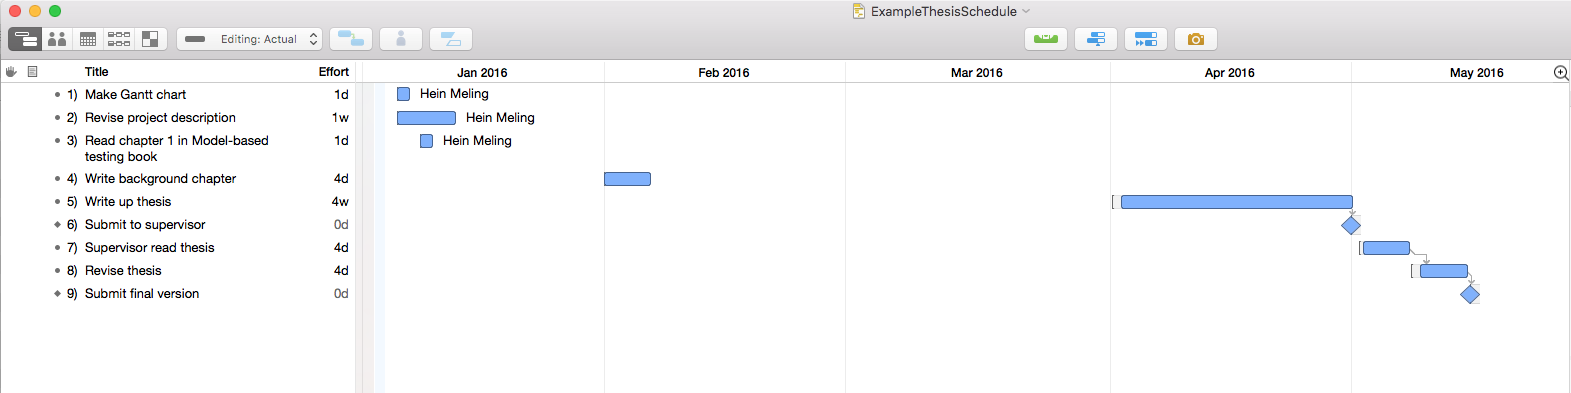
\includegraphics[scale=0.25]{fig/gantt-example}
 \end{center}
\end{frame}


\begin{frame}
\frametitle{Project Description}
\begin{block}{}
 \begin{itemize}
  \item Project descriptions are in some cases a bit vague
  \item Project proposer does not always know what he/she wants
  \item Write your own version
  \item Headings:
  \begin{itemize}
  	\item Background
	\item Motivation
	\item Objectives
	\item Gantt Chart with Tasks and Milestones
  \end{itemize}
  \item Submit project description by \textbf{Monday January 21}
 \end{itemize}
\end{block}
\end{frame}


\begin{frame}
\frametitle{Project Description}
\begin{block}{}
\begin{columns}

\begin{column}{.5\textwidth}
\begin{figure}[htbp]
\centering

\includegraphics[scale=0.2]{fig/p1}
\end{figure}
\end{column}

\begin{column}{.5\textwidth}
\begin{figure}[htbp]
\centering
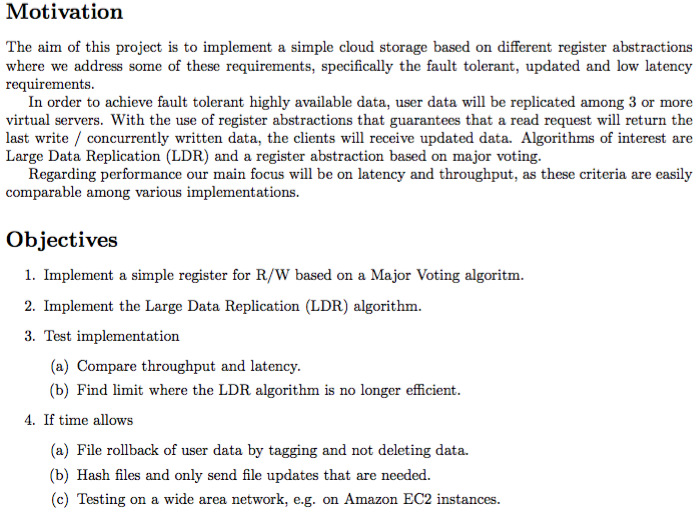
\includegraphics[scale=0.25]{fig/p2}
\end{figure}
\end{column}

\end{columns}
\end{block}
\end{frame}


\begin{frame}
\frametitle{Work Process}
\begin{block}{}
 \begin{itemize}
  \item Individual meetings (approx. 1 hour)
  \item Group meetings (approx. 2 hours)
  \item Reading group (approx. 1 hour)
 \end{itemize}
\end{block}
\end{frame}


\begin{frame}
\frametitle{Work Process: Review Expectations}
\begin{block}{}
 \begin{itemize}
  \item Your advisor will read and comment on your report:
  \begin{itemize}
  	\item First deliverable - partial review
  	\item Second deliverable - full review
	\item No feedback on the final report
  \end{itemize}
  \item In some cases: review code 
  \item Your Advisor's expectation to deliverables:
  \begin{itemize}
  	\item No spelling mistakes that can be caught by the spellchecker!
	\item Reasonable formatting; it should look nice!
  \end{itemize}
  % \item Will help as much as I can by email or Slack
 \end{itemize}
\end{block}
\end{frame}


\begin{frame}
\begin{block}{When Attending a Conference or Summer/Winter School}
 \begin{itemize}
  \item Make connections
  \begin{itemize}
  	\item At least 5 other students
	\item At least 3 speakers/professors
  \end{itemize}
  \item Tell them your plans and ideas and solicit their feedback.
  \begin{itemize}
  	\item Prepare a pitch; a few short sentences that are representative and memorable.
  \end{itemize}
  \item Make notes about their research/personal interests in a journal (include their picture).
  \item Don't do it while talking with them, but afterwards, as soon as it is appropriate.
  \item Then next time you have a chance to meet them (the next conference), read your notes before traveling. You have a higher chance of remembering them, and you give a good impression in that you remembered them. They will start to remember you!
 \end{itemize}
\end{block}
\end{frame}

\begin{frame}
\begin{block}{When to Start Writing?}
 \begin{itemize}
  \item<2-> Today!
  \item<2-> You can set up the document 
  \item<2-> Prepare a disposition (fill in the headings)
  \item<2-> You can always change things later
 \end{itemize}
\end{block}
\end{frame}


\begin{frame}
\begin{block}{How to structure the thesis report}
 % Talk to each bullet here:
 \begin{itemize}
  \item Abstract (300-500 words)
  \item Introduction (3-5 pages)
  \begin{itemize}
  	\item Motivate why your topic is important; summarize idea and results
	\item Important chapter
  \end{itemize}
  % Explain that intro is important; it is what makes the reader decide if it is worth their time
  \item Background, Technology Review, Related Work (10-20 p.)
  % Explain difference between background and related work
  \item Design, Model, Architecture (10-30 p.)
  \item Implementation (10-20 p.)
  \begin{itemize}
   \item Technical details of interest, optimizations, algorithms, ...
   \item Don't explain every bit of code; only the interesting parts
  \end{itemize}
  \item Evaluation, Discussion, Insights (10-30 p.)
  \item Conclusion (300-500 words)
  \begin{itemize}
  	\item Tie the results back to what you promised in the introduction
  \end{itemize}
 \end{itemize}
\end{block}
\end{frame}


% \begin{frame}
% \begin{block}{How to structure the project report}
%  \begin{itemize}
% 	\item Same as for thesis report
% 	\begin{itemize}
% 		\item Except scaled down to 10-16 pages.
% 	\end{itemize}
% 	\item Double column format.
%  \end{itemize}
% \end{block}
% \end{frame}


\begin{frame}
\begin{block}{Tips for the report content}
 \begin{itemize}
  \item Name chapters appropriately; other names than those on previous slide is ok.
  \item Start Chapter/Section with a brief summary of what the reader can expect to learn from reading it.
  \begin{itemize}
   \item Thus far, we have presented Replacement for a single Paxos instance. In this section, we explain how to apply Replacement to an RSM that executes a sequence of Paxos instances.
  \end{itemize}
  \item Insert paragraph breaks (avoid too long paragraphs)
  % \item 
 \end{itemize}
\end{block}
\end{frame}


\begin{frame}
\begin{block}{How to Work?}
 \begin{itemize}
  \item<2-> Switch between coding and writing!
  \item<3-> Expect to rewrite everything you write; 
  \begin{itemize}
  	\item<3-> So don't spend time making it perfect 
  \end{itemize}
  \item<4-> Iterate to improve report to make it perfect
  \item<5-> Why work this way?
  \begin{itemize}
	\item<6-> Two modes of thinking
  	\item<6-> Makes you think differently about the problem 
  \end{itemize}
 \end{itemize}
\end{block}
\end{frame}


\begin{frame}
\begin{block}{Specification: Thinking Before Coding}
 \begin{itemize}
  \item Write specifications:
  \begin{itemize}
  	\item high-level specification of system
	\item low-level specification for each function
  \end{itemize}
  \item Textual specifications are fine!
  \item Also: Express ideas in diagrams and figures
  \item Simplicity
 \end{itemize}
\end{block}
\end{frame}


\begin{frame}
\begin{block}{Modeling Languages}
 \begin{itemize}
  \item Unified Modeling Language (UML)
  \begin{itemize}
	\item Use Case Diagrams
  	\item \textbf{Class Diagrams} (Entity Relation)
	\item \textbf{Sequence Charts}
	\item \textbf{State Machine Diagrams}
  \end{itemize}
  \item \textbf{Flow Charts}
  \item Work Flow Diagrams
  \item Data Flow Diagrams
  \item Wireframe / UI Mockups
  \item Infographics
 \end{itemize}
\end{block}
\end{frame}


\begin{frame}
\begin{block}{Tools}
 \begin{itemize}
  \item git and github
  \item Dropbox
  \item LaTeX/bibtex for the report
  \item Slack for chat rooms
 \end{itemize}
\end{block}
\end{frame}

\begin{frame}
\begin{block}{Quick Guide to git Command Line}
 \begin{itemize}
  \item git clone \pname{repo-link from github}
  \item git add \pname{new-file}
  \item git commit \quad (supply commit message)
  \item git push \quad (send changes to github)
  \item git fetch --all \quad (get changes from github, e.g. by other team members)
  \item git merge \quad (merge changes from github with local branch)
 \end{itemize}
\end{block}
\end{frame}

\begin{frame}
\begin{block}{Quick Guide to git Command Line}
 \begin{itemize}
  \item git pull \quad (alternative to fetch and merge, but causes merge commits that distort the history of changes when not necessary)
  \item git diff \quad (view your changes before commit)
  \item git diff --word-diff \quad (view your changes before commit)
  \item git log \quad (see log of all commits)
 \end{itemize}
\end{block}
\end{frame}


\begin{frame}
\begin{block}{Best Practices: GitHub and LaTeX}
 \begin{itemize}
  \item Naming folders (under bbchain repo):
  \begin{itemize}
  	\item consistent naming; lower-case; think of a good name!
	\item papers/\pname{project-name}/\pname{conference-name}
	\item Example: papers/blockchain-storage/icdcs2020
  \end{itemize}
  \begin{itemize}
  	\item In root folder:
	\begin{itemize}
		\item main.tex
		\item main.bib
		\item \pname{template files for conference/journal}
		\item .gitignore \quad (Use GitHub's TeX template)
	\end{itemize}
	\item In subfolders:
	\begin{itemize}
		\item tex/ \quad fig/ \quad alg/ \quad plots/
	\end{itemize}
	\item Do not commit generated files, including main.pdf
	\begin{itemize}
		\item Include such files in .gitignore
	\end{itemize}
  \end{itemize}
  \end{itemize}
\end{block}
\end{frame}

\begin{frame}
\begin{block}{Publishing}
 \begin{itemize}
  \item Target top conferences
  \item Better to have 1 strong publication at a top conference 
        than 4 at low-tier conferences
  \item People will look at where you published
  \item In Computer Science (systems), ACM and USENIX venues often considered more prestigious than IEEE; there are some exceptions of course
  \item Better to take a few rejects than to submit to easy places.
 \end{itemize}
\end{block}
\end{frame}

\begin{frame}
\begin{block}{Publishing: Plan the Process}
 \begin{itemize}
  \item Pick target conference (deadline given)
  \item Set milestones for intermediate results and subgoals
  \item Timeframe between 3-6 months
  \item Again: use Gantt chart
  \item Revise plan once every two weeks (approx)
 \end{itemize}
\end{block}
\end{frame}

\begin{frame}
\begin{block}{Meeting Setup}
 \begin{itemize}
  \item Individual meetings weekly (1 hour per student)
  \item 
  \item Set milestones for intermediate results and subgoals
  \item Timeframe between 3-6 months
  \item Again: use Gantt chart
  \item Revise plan once every two weeks (approx)
 \end{itemize}
\end{block}
\end{frame}

\begin{frame}
\frametitle{Conference Schedule}
 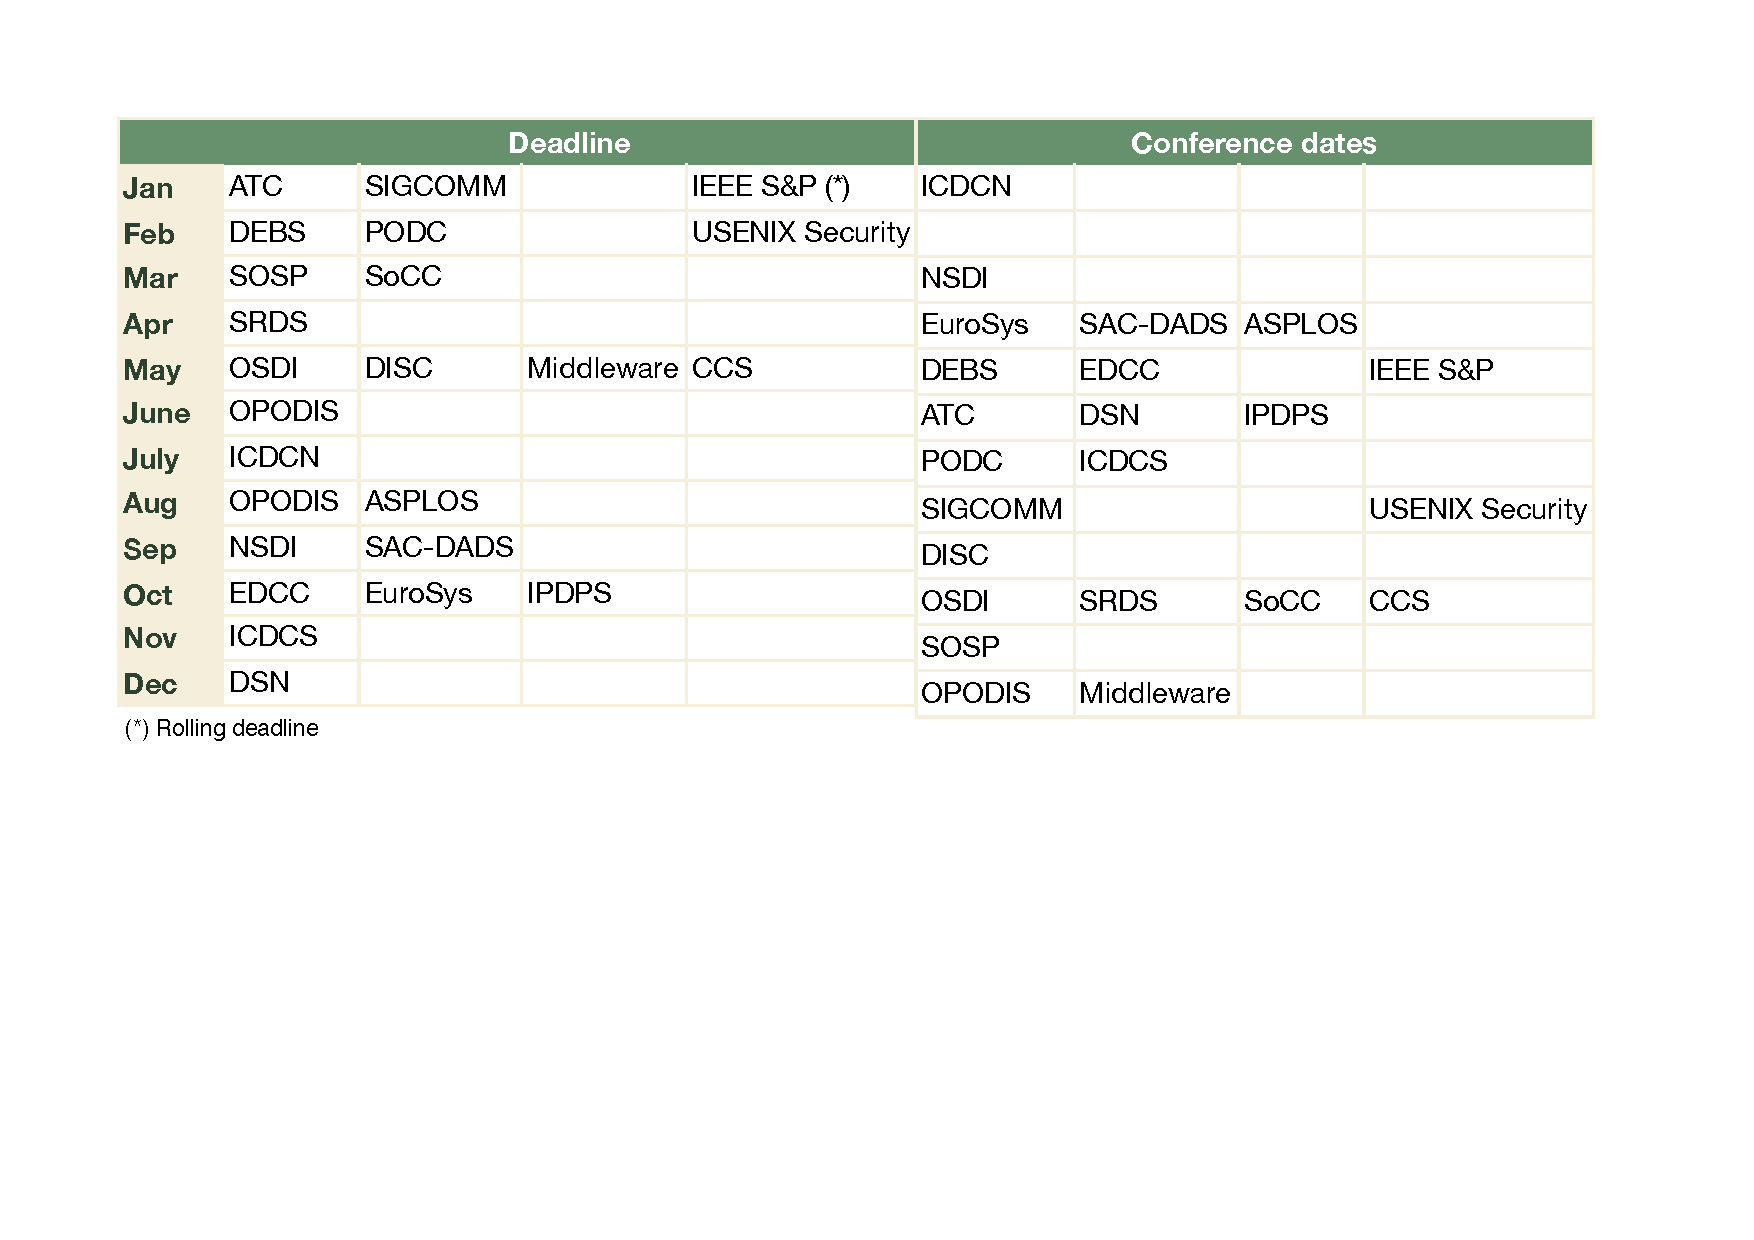
\includegraphics[scale=0.48]{fig/ConferenceSchedule}
\end{frame}

\begin{frame}
\begin{block}{Conclusions}
 \begin{itemize}
  \item We have high expectations
  \item We want you to succeed!
 \end{itemize}
\end{block}
\end{frame}


\end{document}
